\usetikzlibrary{calc}
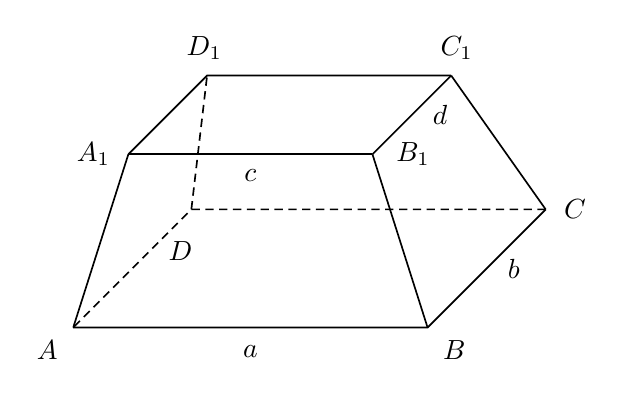
\begin{tikzpicture}[x=1cm,y=1cm,line width=.6pt,font=\normalsize]
\coordinate (A) at (0.0000000000,0.0000000000);
\coordinate (B) at (4.5000000000,0.0000000000);
\coordinate (C) at (6.0000000000,1.5000000000);
\coordinate (D) at (1.5000000000,1.5000000000);
\coordinate (A1) at (0.7000000000,2.2000000000);
\coordinate (B1) at (3.8000000000,2.2000000000);
\coordinate (C1) at (4.8000000000,3.2000000000);
\coordinate (D1) at (1.7000000000,3.2000000000);
\draw (A) -- (B) -- (C);
\draw[densely dashed] (C)--(D)--(A);
\draw[densely dashed] (D) -- (D1);
\draw (A) -- (A1);
\draw (B) -- (B1);
\draw (C) -- (C1);
\draw (A1) -- (D1) -- (C1);
\draw (A1) -- (B1);
\draw (B1) -- (C1);
\node[anchor=north east,xshift=-2pt,yshift=-1pt] at (A) {$A$};
\node[anchor=north west,xshift=2pt,yshift=-1pt] at (B) {$B$};
\node[anchor=west,xshift=3pt] at (C) {$C$};
\node[anchor=north east,xshift=4pt,yshift=-8pt] at (D) {$D$};
\node[anchor=east,xshift=-3pt] at (A1) {$A_{1}$};
\node[anchor=west,xshift=5pt,yshift=0pt] at (B1) {$B_{1}$};
\node[anchor=south,xshift=2pt,yshift=2pt] at (C1) {$C_{1}$};
\node[anchor=south,xshift=-1pt,yshift=2pt] at (D1) {$D_{1}$};
\node[anchor=north,yshift=-3pt] at ($(A)!0.5!(B)$) {$a$};
\node[anchor=west,xshift=4pt] at ($(B)!0.5!(C)$) {$b$};
\node[anchor=north,yshift=-2pt] at ($(A1)!0.5!(B1)$) {$c$};
\node[anchor=west,xshift=4pt] at ($(B1)!0.5!(C1)$) {$d$};
\end{tikzpicture}
